\documentclass[a4paper,11pt]{book}
%\documentclass[a4paper,twoside,11pt,titlepage]{book}
\usepackage{listings}
\usepackage[utf8]{inputenc}
\usepackage[spanish]{babel}

% \usepackage[style=list, number=none]{glossary} %
%\usepackage{titlesec}
%\usepackage{pailatino}
\usepackage[table,xcdraw]{xcolor}
%\decimalpoint
\usepackage{dcolumn}
\usepackage{float}
\newcolumntype{.}{D{.}{\esperiod}{-1}}
\makeatletter
%\addto\shorthandsspanish{\let\esperiod\es@period@code}
\makeatother


%\usepackage[chapter]{algorithm}
\RequirePackage{verbatim}
%\RequirePackage[Glenn]{fncychap}
\usepackage{fancyhdr}
\usepackage{graphicx}
\usepackage{afterpage}

\usepackage{longtable}

\usepackage[pdfborder={000}]{hyperref} %referencia

% ********************************************************************
% Re-usable information
% ********************************************************************
\newcommand{\myTitle}{Tarea 3 - Evaluación Continua\xspace}
\newcommand{\myDegree}{MÁSTER EN INVESTIGACIÓN EN INGENIERÍA DE SOFTWARE Y
SISTEMAS INFORMÁTICOS\xspace}
\newcommand{\myName}{César Hugo Bárzano Cruz\xspace}
\newcommand{\myProf}{Nombre Apllido1 Apellido2 (tutor1)\xspace}
\newcommand{\myOtherProf}{Nombre Apllido1 Apellido2 (tutor2)\xspace}
%\newcommand{\mySupervisor}{Put name here\xspace}
\newcommand{\myFaculty}{ Universidad Nacional de Educación a Distancia\xspace}
\newcommand{\myFacultyShort}{UNED-Facultad de informática\xspace}
\newcommand{\myDepartment}{\xspace}
\newcommand{\myUni}{\protect{ Universidad Nacional de Educación a Distancia}\xspace}
\newcommand{\myLocation}{Madrid\xspace}
\newcommand{\myTime}{\today\xspace}
\newcommand{\myVersion}{Version 0.1\xspace}


\hypersetup{
pdfauthor = {\myName hugobarzano@gmail.com},
pdftitle = {\myTitle},
pdfsubject = {},
pdfkeywords = {},
pdfcreator = {LaTeX con el paquete TEXmaker},
pdfproducer = {pdflatex}
}

%\hyphenation{}


%\usepackage{doxygen/doxygen}
%\usepackage{pdfpages}
\usepackage{url}
\usepackage{colortbl,longtable}
\usepackage[stable]{footmisc}
%\usepackage{index}

%\makeindex
%\usepackage[style=long, cols=2,border=plain,toc=true,number=none]{glossary}
% \makeglossary

% Definición de comandos que me son tiles:
%\renewcommand{\indexname}{Índice alfabético}
%\renewcommand{\glossaryname}{Glosario}

\pagestyle{fancy}
\fancyhf{}
\fancyhead[LO]{\leftmark}
\fancyhead[RE]{\rightmark}
\fancyhead[RO,LE]{\textbf{\thepage}}
\renewcommand{\chaptermark}[1]{\markboth{\textbf{#1}}{}}
\renewcommand{\sectionmark}[1]{\markright{\textbf{\thesection. #1}}}

\setlength{\headheight}{1.5\headheight}

\newcommand{\HRule}{\rule{\linewidth}{0.5mm}}
%Definimos los tipos teorema, ejemplo y definición podremos usar estos tipos
%simplemente poniendo \begin{teorema} \end{teorema} ...
\newtheorem{teorema}{Teorema}[chapter]
\newtheorem{ejemplo}{Ejemplo}[chapter]
\newtheorem{definicion}{Definición}[chapter]

\definecolor{gray97}{gray}{.97}
\definecolor{gray75}{gray}{.75}
\definecolor{gray45}{gray}{.45}
\definecolor{gray30}{gray}{.94}

\lstset{ frame=Ltb,
     framerule=0.5pt,
     aboveskip=0.5cm,
     framextopmargin=3pt,
     framexbottommargin=3pt,
     framexleftmargin=0.1cm,
     framesep=0pt,
     rulesep=.4pt,
     backgroundcolor=\color{gray97},
     rulesepcolor=\color{black},
     %
     stringstyle=\ttfamily,
     showstringspaces = false,
     basicstyle=\scriptsize\ttfamily,
     commentstyle=\color{gray45},
     keywordstyle=\bfseries,
     %
     numbers=left,
     numbersep=6pt,
     numberstyle=\tiny,
     numberfirstline = false,
     breaklines=true,
   }

% minimizar fragmentado de listados
\lstnewenvironment{listing}[1][]
   {\lstset{#1}\pagebreak[0]}{\pagebreak[0]}

\lstdefinestyle{CodigoC}
   {
	basicstyle=\scriptsize,
	frame=single,
	language=C,
	numbers=left
   }
\lstdefinestyle{CodigoC++}
   {
	basicstyle=\small,
	frame=single,
	backgroundcolor=\color{gray30},
	language=C++,
	numbers=left
   }


\lstdefinestyle{Consola}
   {basicstyle=\scriptsize\bf\ttfamily,
    backgroundcolor=\color{gray30},
    frame=single,
    numbers=none
   }


\newcommand{\bigrule}{\titlerule[0.5mm]}
\usepackage{enumitem}


%Para conseguir que en las páginas en blanco no ponga cabecerass
\makeatletter
\def\clearpage{%
  \ifvmode
    \ifnum \@dbltopnum =\m@ne
      \ifdim \pagetotal <\topskip
        \hbox{}
      \fi
    \fi
  \fi
  \newpage
  \thispagestyle{empty}
  \write\m@ne{}
  \vbox{}
  \penalty -\@Mi
}
\makeatother

\usepackage{pdfpages}

\begin{document}
\begin{titlepage}
 
 
\newlength{\centeroffset}
\setlength{\centeroffset}{-0.5\oddsidemargin}
\addtolength{\centeroffset}{0.5\evensidemargin}
\thispagestyle{empty}

\noindent\hspace*{\centeroffset}\begin{minipage}{\textwidth}

\centering

\includegraphics[width=0.7\textwidth]{imagenes/Logo-uned.jpg}\\[1.1cm]


{\Huge\bfseries Máster Universitario En Investigación En Ingeniería De Software Y Sistemas Informáticos\\
}
\noindent\rule[-1ex]{\textwidth}{3pt}\\[3.5ex]
{\large\bfseries Sistemas De Percepción Visual}
\end{minipage}

\vspace{2.5cm}
\noindent\hspace*{\centeroffset}\begin{minipage}{\textwidth}
\centering

\textbf{Autor}\\ {César Hugo Bárzano Cruz}\\[2.5ex]


\includegraphics[width=0.3\textwidth]{imagenes/Logo-master.png}\\[0.1cm]
\textsc{Trabajo Final de la asignatura}\\
\textsc{---}\\
2018/2019
\end{minipage}
%\addtolength{\textwidth}{\centeroffset}
%\vspace{\stretch{2}}
\end{titlepage}




%\frontmatter
\tableofcontents
\listoffigures
%\listoftables

%
%\mainmatter
%\setlength{\parskip}{5pt}

%\input{capitulos/01_Introduccion}


\chapter{Introducción}

El presente documento representa la memoria formal para evaluación continua del Trabajo Final de la asignatura  Sistemas De Percepción Visual. Dicho trabajo práctico aborda el "Reconocimiento Facial" como problema de aplicación concreta. En los siguientes capítulos se mostrará el estado del arte en cuanto a esta disciplina, se abordarán ejemplos concretos de aplicación, posibles aplicaciones de negocio. 

De manera adicional, y a modo de prototipo, este trabajo incluye un ejemplo de aplicación practica de un sistema se percepción visual, concreta mente un centinela capaz de aprender y reconocer caras. El objetivo de este prototipo  es mostrar el procesamiento necesario para reconocimiento facial así como mejorar su aprendizaje y detección de nuevos rostros humanos

\chapter{El Problema}

El reconocimiento facial es un método para identificar y verificar a identidad de un individuo mediante su rostro. Los sistemas de percepción visual basados en el reconocimiento de caras pueden ser usados para identificar a las personas en fotos, vídeo, tiempo real o incluso desde dispositivos móviles.  El reconocimiento facial es considerada una técnica biométrica. La biometria se usa para identificar y autenticar a una persona usando un conjunto de datos reconocibles y verificables únicos y específicos de esa persona.  Las técnicas de reconocimiento facial pueden clasificarse según el siguiente diagrama: 

\begin{figure}[H]  
\centering 
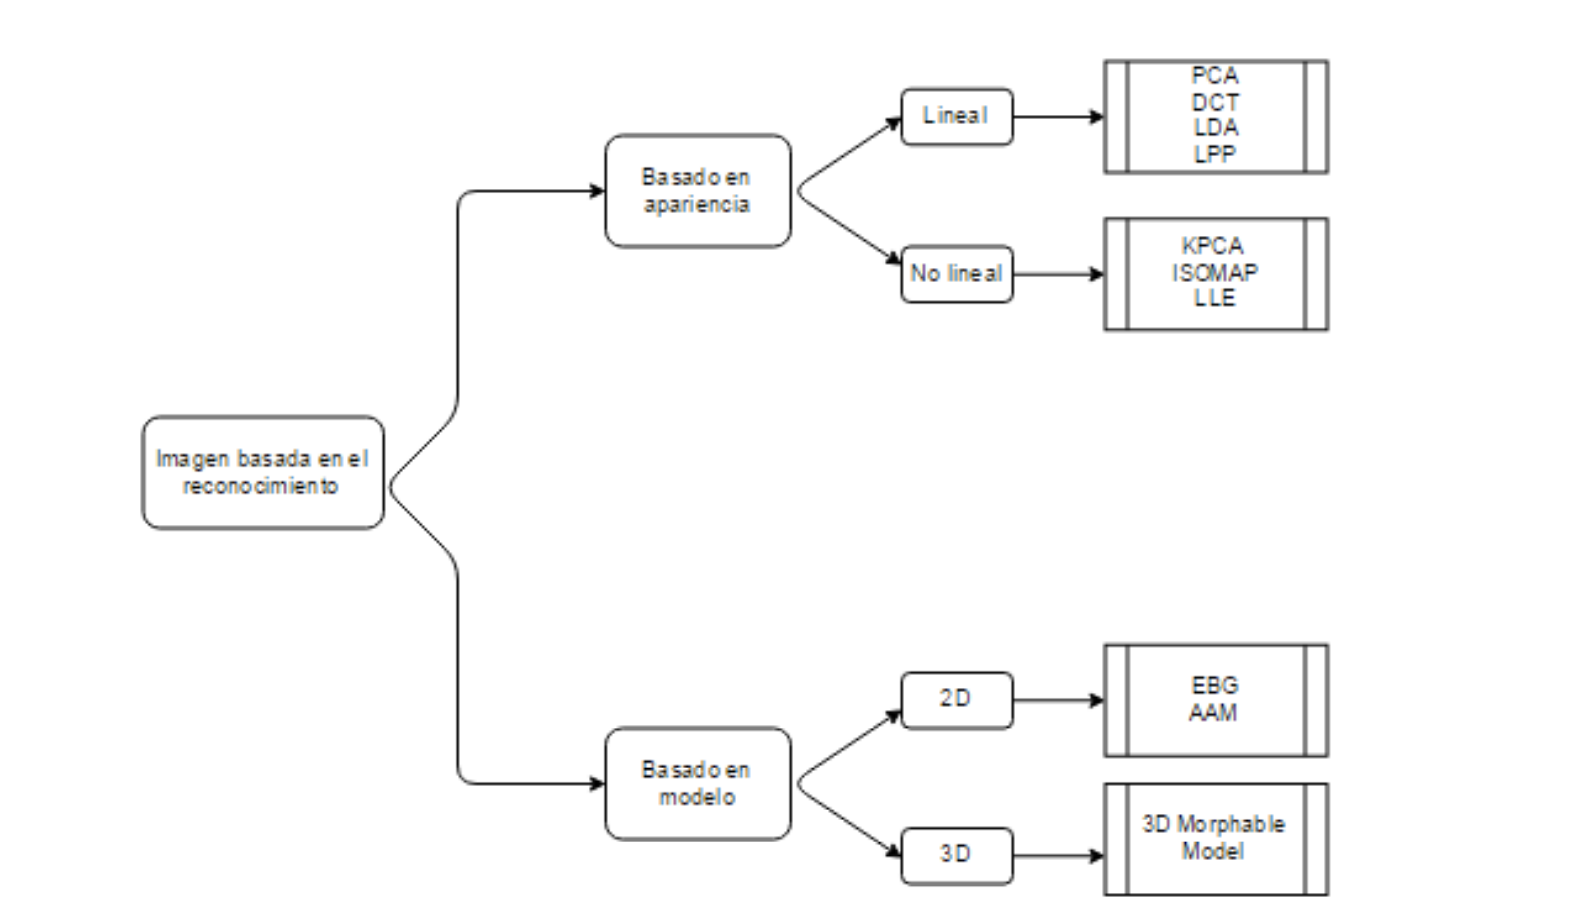
\includegraphics[scale=0.45]{imagenes/tecnicas.png}
\caption{ El problema: Técnicas de Reconocimiento Facial}  
\end{figure} 

\section{Técnicas Reconocimiento Facial }

\subsection{PCA: PRINCIPAL COMPONENT ANALYSIS}

El objetivo de esta técnica consiste en representar una imagen en términos de un
sistema de coordenadas óptimo reduciendo el número final de componentes. Con PCA se consigue encontrar los vectores que mejor representan la distribución que existe en un grupo de imágenes. 

PCA esta basado en la Transformada de Karhunen-Loeve\cite{loeve}  permite representar una imagen de una cara usando una base que se ha conseguido a partir de muchas observaciones de diferentes caras. 

\subsection{LDA: LINEAR DISCRIMINANT ANALYSIS}

LDA pretende convertir un problema de alta dimensionalidad en uno de baja
dimensionalidad. Esta técnica se basa en aumentar la distancia existente entre clases para conseguir una mayor discriminación entre ellas.\cite{pIborra}
La gran diferencia entre LDA y PCA es que esta técnica requiere de una supervisión durante el entrenamiento mientras que PCA utiliza un entrenamiento no supervisado.

LDA utiliza diferentes aproximaciones como pseudo-inverse LDA\cite{ravi}, que utiliza la pseudo-inversa de la matriz de covarianza en lugar de su inversa

\subsection{LPP: Locality Preserving Projections}

Es un algoritmo lineal que realiza una reducción dimensional de los datos. Al tratarse de un algoritmo lineal es rápido y útil para aplicaciones prácticas. 

LPP\cite{he} conserva la estructura de datos local.  Consiguiendo así que los "vecinos" para un dato en concreto serán los mismos en el espacio original, de alta dimensionalidad, y en el nuevo subespacio de baja dimensionalidad. Al conservarse la estructura local de los datos, las
imágenes pertenecientes a un mismo individuo estarán cercanas entre si y
alejadas de las de otros individuos, es decir, hay una discriminación entre
clases. 

Para conservar la estructura local de los datos se hace uso de un grafo de
adyacencias que incluye información de la estructura de los datos. Este grafo consiste en la creación de una matriz de tamaño NxN, donde N es el número de imágenes, que tiene asignados unos pesos dependiendo de si los elementos i y j son vecinos o no. 

\subsection{DCT: Discrete Cosine Transform}

La DCT es una transformación que representa una secuencia finita de datos
como la suma de una serie de funciones cosenoidales oscilando a diferentes
frecuencias. Este método no necesita ser entrenado con imágenes del
mismo tipo a las que se van a usar sino que simplemente se transforman
directamente las imágenes. 

\subsection{DCT por Bloques }

Este método realiza una mezcla de las técnicas basadas en la apariencia y las
basadas en modelos, en concreto, hace uso de la misma metodología que el
método DCT pero aplicado de forma distinta.  

Este sistema hace uso parcial de los sistemas basados en modelos porque
requiere de la localización de alguna característica facial.  

\section{Sistemas Reconocimiento Facial }

\subsection{ Eigenfaces}

Es un algoritmo\cite{turk}  de reconocimiento facial basado en el análisis por componentes principales. Identifica patrones en las imágenes y clasifica a cada individuo en función de las coordenadas obtenidas en el subespacio que se forma a través de estas componentes.

Este algoritmo necesita de un conjunto de entrenamiento o caras de personas
que harán el papel de vectores de observación. Estos vectores vendrán determinamos por cada pixel de la imagen.
Para poder utilizar este algoritmo, todas las imágenes han de tener el mismo tamaño. Todas las imágenes deben tener n = WxH píxeles, donde W es el ancho de la imagen y H la altura. Por lo tanto, cada imagen es representada como un punto en un subespacio vectorial de N dimensiones.

\subsection{ Fisherface}

Este sistema\cite{vs} se pretende maximizar la distancia entre clases y minimizar la distancia dentro de la misma clases. Consiste en usar LDA para reducir la
dimensión de los datos a N – C , donde N es el número de imágenes y C es el número de individuos que se encuentran en el conjunto de entrenamiento, también llamado clases. 

\chapter{Estado del Arte}

En el estudio Facial Recognition Market by Technology\cite{market} publicado en 2016 se estimó que para el 2022 el nicho de negocio relacionado con el reconocimiento facial generaria mas de 9.000 millones de ingresos, con una tasa de crecimiento anual del 21.3\% dureante el perido 2016-2022. Las principales sectores económicos de aplicación de técnicas de reconocimiento facial se pueden agrupar en tres categorías principales: 

\section{Seguridad}
Sector económico liderado por una mayor actividad para combatir el crimen y el terrorismo, así como la competencia económica y empresarial. 

\begin{enumerate}
\item El reconocimiento facial se utiliza al emitir documentos de identidad y, la mayoría de las veces, se combina con otras tecnologías biométricas, como las huellas dactilares.

\item La coincidencia de rostros se utiliza en las verificaciones fronterizas para comparar la foto de un pasaporte biométrico digitalizado con el rostro del portador de dicho pasaporte. 


\item La biometria facial también se puede utilizar en controles policiales, aunque su uso está rigurosamente controlado en Europa

\item La biometría también es utilizada por corporaciones gubernamentales, empresas y algunas universidades como método de control y acceso a ciertas áreas o equipos de trabajo. 

\end{enumerate}

\section{Salud}

En esta área se han realizado importantes avances. Gracias al aprendizaje profundo y al análisis de rostros es posible:
\begin{enumerate}
\item Rastrear el uso de medicamentos de un paciente con más precisión
\item Detectar enfermedades genéticas, como el síndrome DiGeorge con una tasa de acierto del 96.6\%
\item Apoyar los procedimientos de manejo del dolor y tele-asistencia. 
\item Ayuda en la identificación de personas con cierto nivel de dependencia ante situaciones de desorientación
\end{enumerate}

\section{Marketing}

A través de las imagenes obtenidas de cámaras en tiendas, ahora es posible analizar el comportamiento de los compradores y mejorar el proceso de compra del cliente. Al igual que el sistema diseñado recientemente por Facebook, el personal de ventas recibe información del cliente extraída de los perfiles de las redes sociales para producir respuestas perfectamente personalizadas. El gran almacén estadounidense Saks Fifth Avenue  ya está usando este sistema.

\section{Proyectos de Innovación}

En algunos comercios Estadounidenses pertenecientes a Amazon, se emplean tecnicas de reconocimiento facial junto con técnicas de reconocimiento de modelos para la realización de las compras cotidianas. El sistema identifica al usuario cuando entra en el comerció, va traqueando o reconociendo los objetos que deposita en su cesto para finalmente realizar el cargo correspondiente por la compra cuando el usuario o cliente sale del establecimiento. 

En los comedores para empleados de algunas ciudades financieras del banco BBVA, se permite realizar el pago del menú  diario del comedor mediante reconocimiento facial de la persona que realiza la compra comparada con la base de empleados del propio banco. 


\section{Tecnología}
En marzo de 2018 la Dirección de Ciencia y Tecnología de la Seguridad Nacional de los Estados Unidos, conocida como Biometric Technology Rally\cite{rally}, publicó un ranking sobre el  mejor software de reconocimiento facial disponible en el mercado:

\begin{enumerate}
\item El algoritmo GaussianFace\cite{gaussianface}
	Desarrollado en 2014 por investigadores de la Universidad de Hong Kong logró un nivel de identificación facial del 98.52\% en comparación con el 97.53\% alcanzado por humanos.
	
\item En 2014, Facebook anunció el lanzamiento de su programa DeepFace\cite{deepface} que puede determinar si dos rostros pertenecen a la misma persona, con una tasa de precisión del 97.25\%.

\item En 2015, Google presentó  FaceNet\cite{facenet}, un nuevo sistema de reconocimiento con un nivel de de identificación del 100\% de precisión en la prueba de referencia Labeled Faces in The Wild, y 95\% en la base de datos de rostros de YouTube denominada YouTube Faces DB\cite{youtube}

Esta tecnología se incorpora a Google Photos y se utiliza para clasificar imágenes y etiquetarlas automáticamente en
 función de las personas reconocidas. Demostrando su importancia en el área de la biometría, fue seguido rápidamente por el lanzamiento en línea de una versión de código abierto no oficial conocida como OpenFace
 
 \item En 2018, Ars Technica\cite{ars} informó que Amazon ya está promocionando activamente su servicio de reconocimiento facial basado en la nube llamado Rekognition\cite{aws} para las agencias encargadas del cumplimiento de la ley. La solución podría reconocer hasta 100 personas en una sola imagen y puede realizar coincidencias faciales con bases de datos que contienen decenas de millones de rostros. 
 
\end{enumerate}

\chapter{Aplicación Práctica}

En este capítulo se mostrará un ejemplo practico a modo de ejemplo de aplicación concreta relacionada con el aprendizaje y reconocimiento facial. 

\section{piSentinel}

Como ejemplo concreto de aplicación práctica, se propone la aplicación piSentinel, la cual puede ser encontrada en el siguiente repositorio \url{https://github.com/hugobarzano/piSentinel}

piSentinel consiste en una herramienta en linea de comandos capaz de aprender nuevas caras o buscar caras previamente aprendidas.  Para ello, se consideran dos funciones principales:

\subsection{Aprendizaje o Entrenamiento}

Mediante este comportamiento piSentinel utiliza la web-cam de la máquina en la que se ejecute para detectar y aprender nuevas caras.
Con cada cara aprendida, la aplicación genera 3 ficheros  con la convención de nombre:
\textbf{(nombre\_cara)\_N(indice)\_(fecha)(version).jpg} esto permite a  piSentinel tener mas información sobre la cara, pues cada uno de estos ficheros 
corresponde a la imagen inicial tomada, la cara detectada y otra versión correspondiente a un tamaño menor para facilitar su procesamiento. 

 De manera adicional, la aplicación puede aprender caras nuevas incluyendo  imágenes de caras en  formato jpg y con la convención de nombre: \textbf{(nombre\_cara)\_N(información adicional).jpg}  La aplicación usará \textbf{(nombre\_cara)} para etiquetar a las imágenes que conozca cuando este en modo búsqueda. 

\subsection{Búsqueda o Detección} 

Mediante esta funcionalidad, piSentinel es capaz de detectar caras e identificar las previamente aprendidas. Cuantas mayor sea el número de caras previamente aprendidas, mayor será la precisión del centinela. 

\subsection{Tecnología} 

piSentinel ha sido desarrollado completamente con python3. El centinela hace uso principalmente de las librerias python de visión por computador\cite{picv} y de la librería  face\_recognition\cite{face}. Las dependencias necesarias para ejecutar pySentinel pueden ser consultadas en el fichero de \href{https://github.com/hugobarzano/piSentinel/blob/master/requirements.txt}{ requirements.txt}


\chapter{Caso de Uso}

En este capitulo, se va a realizar un caso de uso con piSentinel en el que se mostrará las funcionalidades de aprendizaje y reconocimiento. 

\section{Aprendizaje}

Para comenzar, vamos a enseñar a piSentinel una cara, la de César Hugo Bárzano Cruz ( yo mismo ). Para ello, se puede ejecutar pySentinel.py con el flag -t (face\_name) para indicar a piSentinel que aprenda la cara de Hugo. 

\begin{lstlisting}
$  python3  piSentinel.py -t Hugo
\end{lstlisting}

\begin{figure}[H]  
\centering 
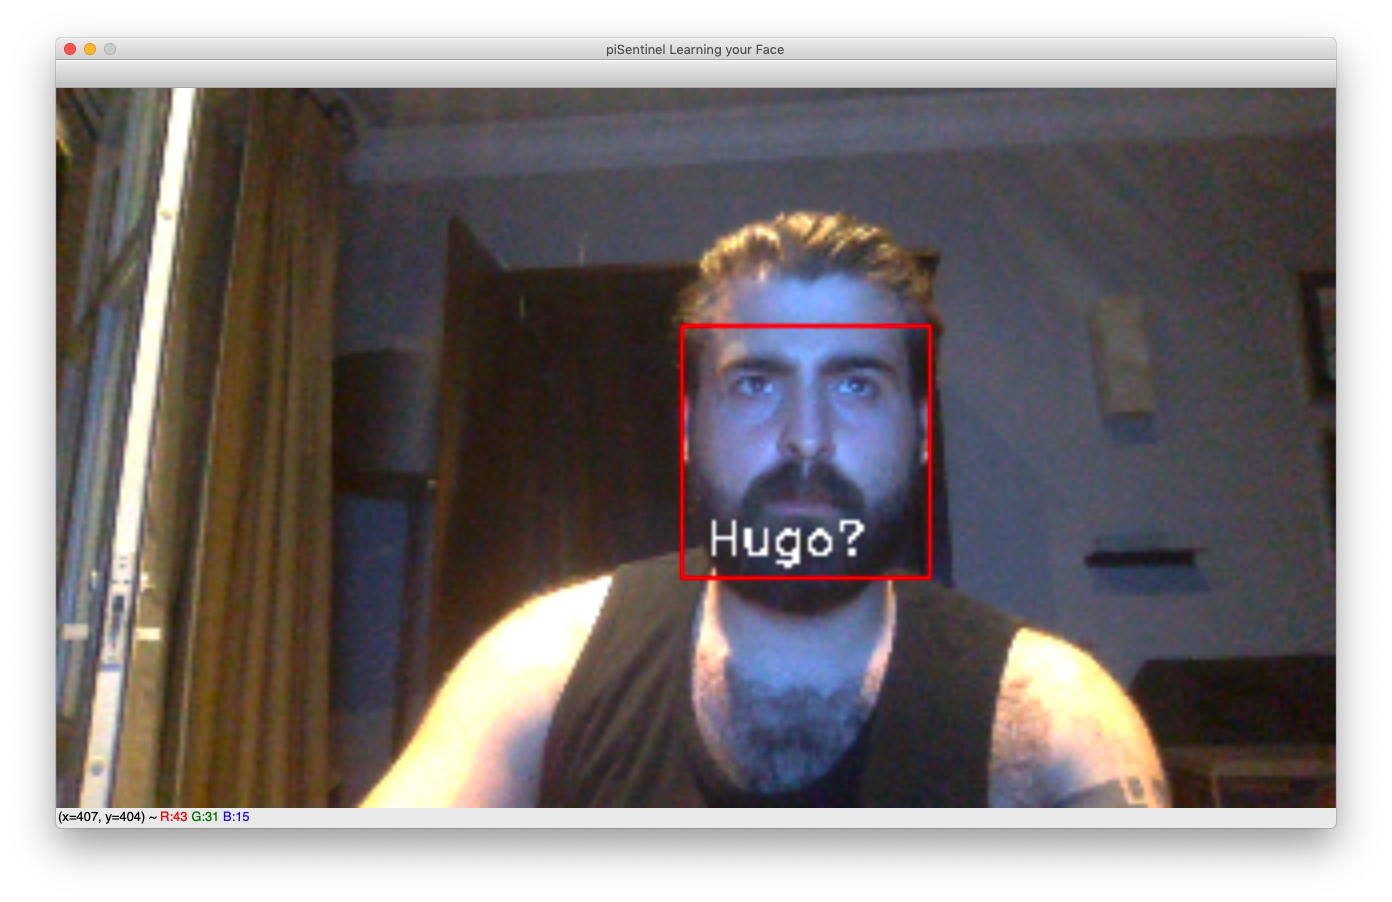
\includegraphics[scale=0.2]{imagenes/dochugo.png}
\caption{ Aprendizaje}  
\end{figure} 

Cuando la aplicación detecte la cara, preguntará si es la cara esperada y al pulsar la tecla "Q" piSentinel capturará el frame y guardará bajo el directorio img/ la información de dicha cara. 

Por ejemplo, para la cara de Hugo, piSentinel generará las siguientes imágenes: 

\subsubsection{Cara detectada}
\begin{figure}[H]  
\centering 
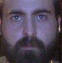
\includegraphics[scale=0.80]{imagenes/Hugo_N0_20190529225417v0.jpg}
\caption{ Aprendizaje: Hugo N0}  
\end{figure} 

\subsubsection{Imagen inicial}
\begin{figure}[H]  
\centering 

\includegraphics[scale=0.30]{imagenes/Hugo_N1_20190529225417v1.jpg}
\caption{ Aprendizaje: Hugo N1 V1}  
\end{figure} 

\subsubsection{Imagen inicial reducida}
\begin{figure}[H]  
\centering 

\includegraphics[scale=0.80]{imagenes/Hugo_N1_20190529225417v2.jpg}
\caption{ Aprendizaje: Hugo N1 V2}  
\end{figure} 

\section{Búsqueda}

La búsqueda de caras conocidas puede llevarse acabo mediante el siguiente comando, indicando el flag -s 

\begin{lstlisting}
$  python3  piSentinel.py -s
\end{lstlisting}

\begin{figure}[H]  
\centering 
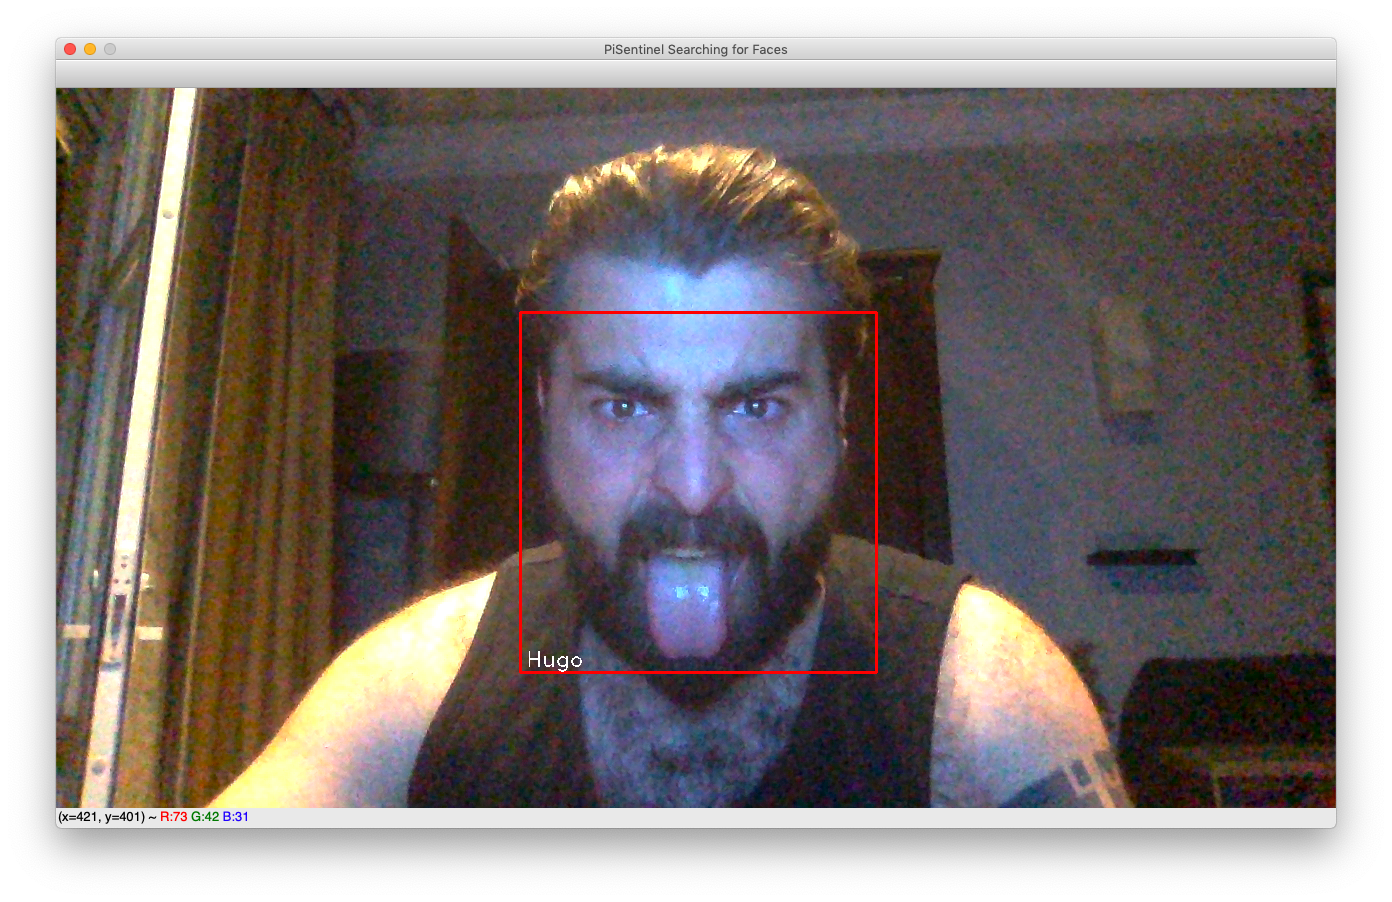
\includegraphics[scale=0.2]{imagenes/doc_hugo2.png}
\caption{ Busqueda: Conocido}  
\end{figure} 

\begin{figure}[H]  
\centering 
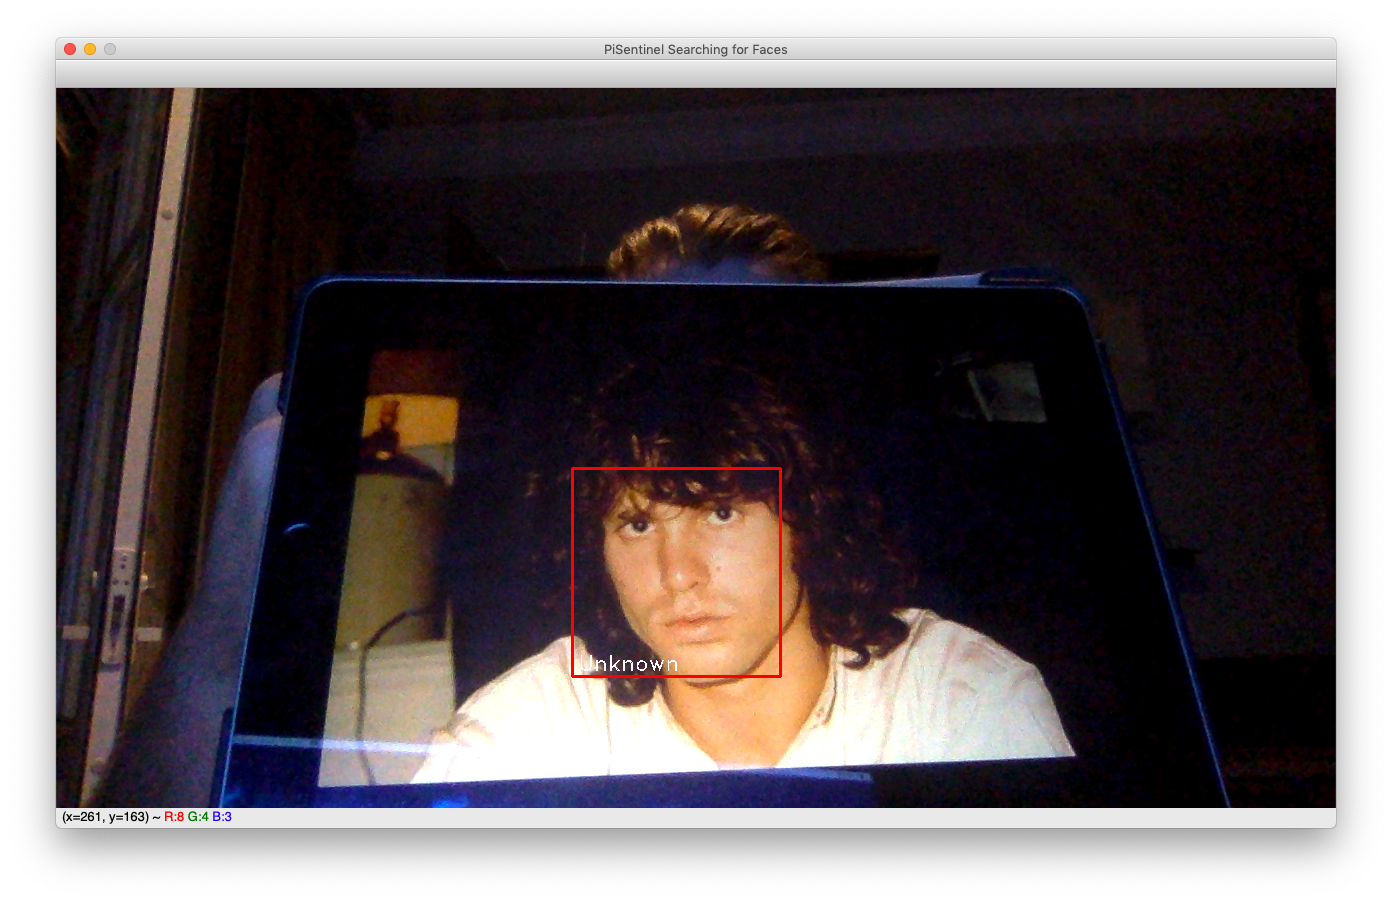
\includegraphics[scale=0.2]{imagenes/doc_jim.png}
\caption{ Busqueda: Desconocido}  
\end{figure} 

\section{Aprendizaje Estático}

De manera adicional y para poder aprender caras con una mayor resolución que la capturada por la web-cam, piSentinel acepta aprender nuevas caras simplemente guardando en el directorio img/ la imagen que se quiera enseñar a la aplicación siguiendo la convención de nombres (nombre\_cara)\_N(información\_adicional). Por ejemplo, si se almacena la siguiente imagen con el nombre Jim\_Morrison\_N0\_static.jpg, en la siguiente ejecución de pySentinel en modo búsqueda, sera capaz de identificar la cara del músico. 

\begin{figure}[H]  
\centering 
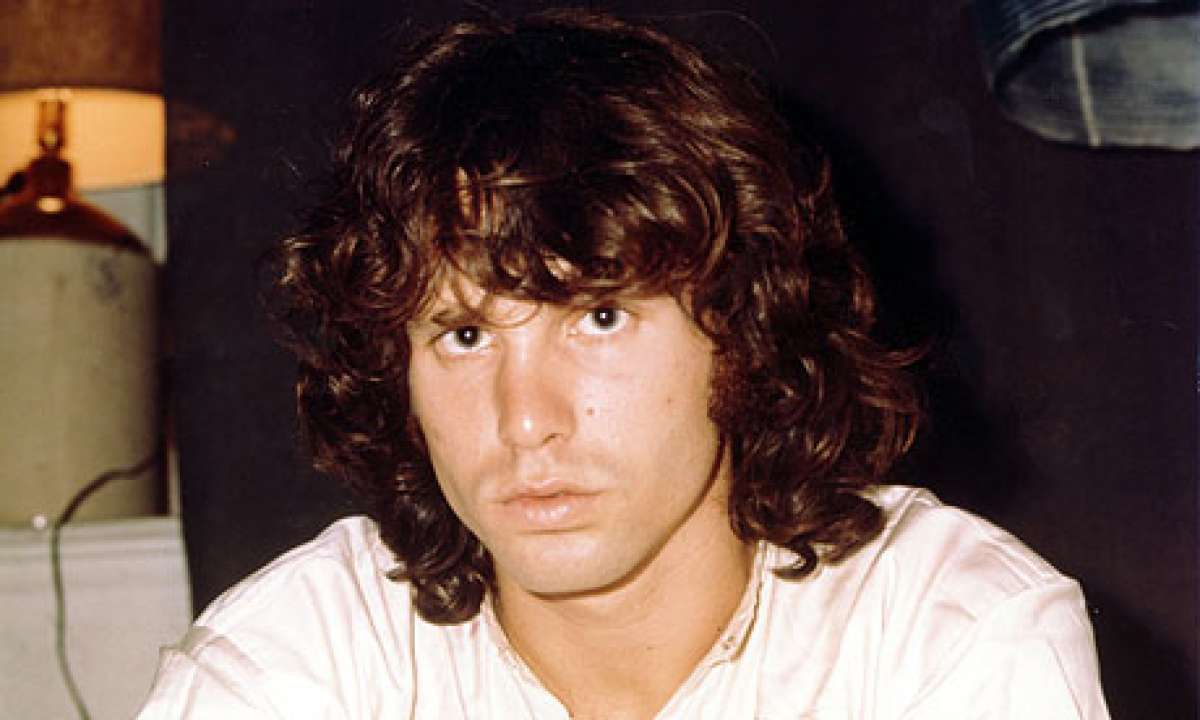
\includegraphics[scale=0.2]{imagenes/Jim_Morrison_N0_static.jpg}
\caption{ Aprendizaje Estático: img/Jim\_Morrison\_N0\_static.jpg }  
\end{figure} 



\begin{figure}[H]  
\centering 
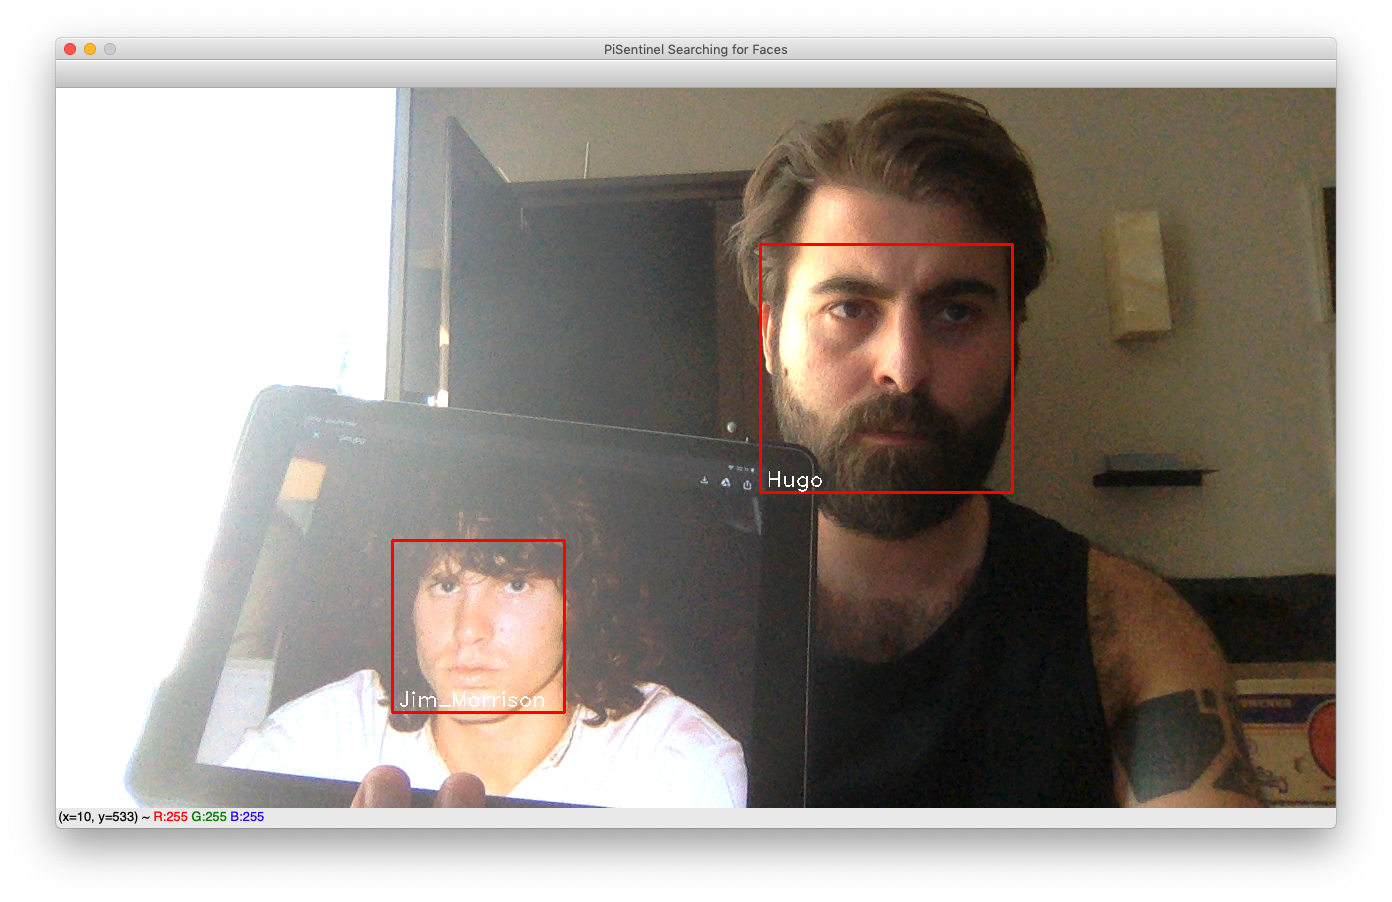
\includegraphics[scale=0.2]{imagenes/static.png}
\caption{ Nuevo ciclo de búsqueda }  
\end{figure} 



\chapter{ Anexo}

Adjunto información solicitada por la Agencia Nacional Evaluadora de los Títulos Oficiales

\begin{figure}[H]  
\centering 
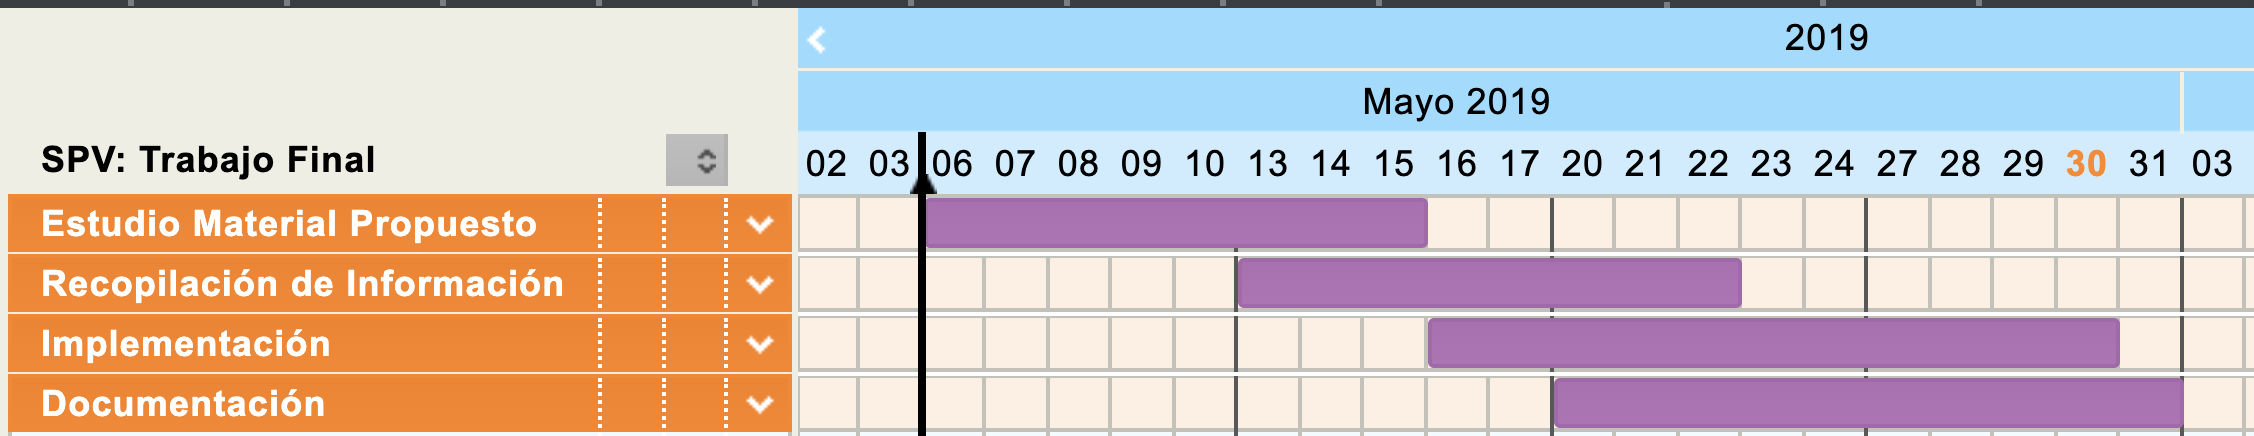
\includegraphics[scale=0.40]{imagenes/gant.png}
\caption{ Anexo: Diagrama Gant}  
\end{figure} 


\begin{thebibliography}{aaaa}

\bibitem{pIborra}
PIborra, Marcelo J. Armengot. Análisis comparativo de métodos basados en subespacios
aplicados al reconocimiento de caras. Valencia- Universitat de València, 2006.

\bibitem{market}
Facial Recognition Market by Technology (2D Facial Recognition, 3D Facial Recognition and Facial Analytics), Component (Hardware and Software) and Application (Homeland Security, Criminal Investigation, ID Management, Physical Security, Intelligent Signage, Photo Indexing and Sorting, Business Intelligence and Photo Indexing and Sorting) - Global Opportunity Analysis and Industry Forecast, 2015 - 2022


\bibitem{rally}
Biometric Technology Rally
https://www.dhs.gov/science-and-technology/biometric-technology-rally

\bibitem{gaussianface}
Surpassing Human-Level Face Verification Performance on LFW with GaussianFace

\bibitem{deepface}
DeepFace - Face Detection, Verification, Recognition and Emotion
https://deepface.ir/

\bibitem{facenet}
FaceNet: A Unified Embedding for Face Recognition and Clustering
https://arxiv.org/abs/1503.03832

\bibitem{youtube}
YouTube Faces Database
https://www.cs.tau.ac.il/~wolf/ytfaces/

\bibitem{ars}
Ars Technica
Serving the Technologist for more than a decade, https://arstechnica.com

\bibitem{aws}
Amazon Rekognition
Easily add intelligent image and video analysis to your applications, https://aws.amazon.com/rekognition

\bibitem{loeve}
M. Kirby and L. Sirovich, “Application of the Karhunen-Loeve procedure for
the characterization of human faces” 

\bibitem{ravi}
 Jieping Ye, Ravi Janardan, Qi Li. “Two-Dimensional Linear Discriminant Analysis”

\bibitem{he}
Xiaofei He and Partha Niyogi. "Locality Preserving Projections"

\bibitem{turk}
Matthew Turk and Allex Pentland
Eigenfaces for Recognition, http://www.face-rec.org/algorithms/PCA/jcn.pdf

\bibitem{vs}
Eigenfaces vs. Fisherfaces:
Recognition Using Class Specic Linear Projection
https://vision.cornell.edu/se3/wp-content/uploads/2014/09/eccv96.pdf

\bibitem{picv}
opencv-python 4.1.0.25
https://pypi.org/project/opencv-python

\bibitem{face}
face\_recognition 1.2.3
https://pypi.org/project/face\_recognition



\end{thebibliography}







%
%
%%\nocite{*}
%\bibliography{bibliografia/bibliografia}\addcontentsline{toc}{chapter}{Bibliografía}
%\bibliographystyle{miunsrturl}
%
%\appendix

%\input{apendices/manual_usuario/manual_usuario}
%%\input{apendices/paper/paper}
%\input{glosario/entradas_glosario}
% \addcontentsline{toc}{chapter}{Glosario}
% \printglossary

\thispagestyle{empty}

\end{document}
